\documentclass{article}
\usepackage{tikz,pgfplots}
\usepackage{tikz-qtree}
\pgfplotsset{compat=1.8}
%\pgfplotsset{colormap={mix}{
%	color(0cm)=(blue);
%	color(1cm)=(green);
%	color(2cm)=(yellow)
%	color(3cm)=(red)}}

\usetikzlibrary{patterns,shadows,trees}

\definecolor{diplom1}{rgb}{0.0 0.4 1.0}
\definecolor{diplom2}{rgb}{0.0 0.0 0.6}
\definecolor{diplom3}{RGB}{153,0,0} %unirot
\definecolor{diplom4}{RGB}{232,215,23}
\definecolor{diplom5}{RGB}{51,37,60}

\definecolor{unirot}{RGB}{153,0,0}
\definecolor{unirot_hell}{RGB}{255,228,225}
\definecolor{lightblue}{RGB}{242.2,249.88,255}

\pgfplotsset{colormap={diplom1s}{
       color(0cm)=(white);
       color(1cm)=(diplom1);
       color(10cm)=(diplom1)}}
\pgfplotsset{colormap={diplom2s}{
       color(0cm)=(white);
       color(1cm)=(diplom1);
       color(2cm)=(diplom2)}}

\tikzset{font=\small,
edge from parent fork down,
level distance=1.75cm,
every node/.style=
    {top color=white,
    bottom color=diplom2!25,
    rectangle,rounded corners,
    minimum height=8mm,
    draw=diplom2!75,
    very thick,
    drop shadow,
    align=center,
    text depth = 0pt
    },
edge from parent/.style=
    {draw=diplom2!50,
    thick
    }}

\begin{document}

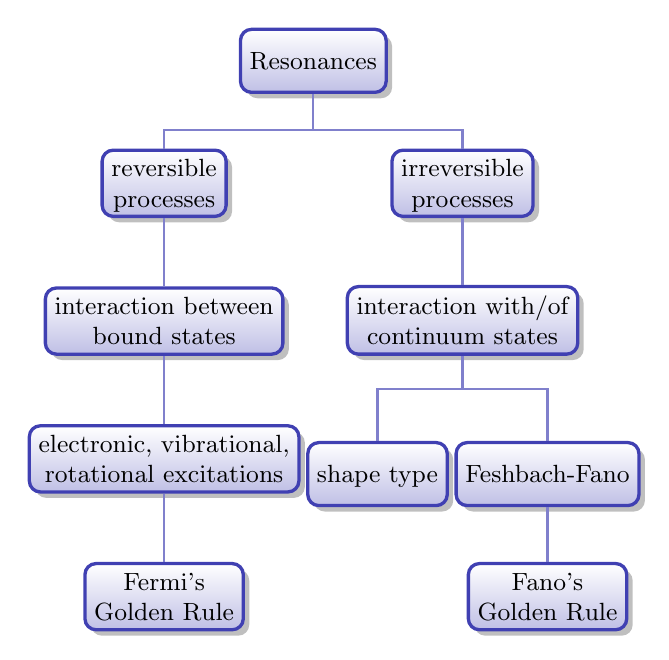
\begin{tikzpicture}[scale=1.0]

\Tree [.Resonances
        [.{reversible\\ processes}
          [.{{interaction between}\\{bound states}}
            [.{{electronic, vibrational,}\\{rotational excitations}}
              [.{{Fermi's}\\{Golden Rule}}
              ]
            ]
          ]
         ] 
        [.{irreversible\\processes}
           [.{{interaction with/of}\\{continuum states}} 
             [.{shape type}
              ]
             [.Feshbach-Fano
               [.{Fano's\\{Golden Rule}}
               ]
              ]
           ]
         ]
]

\end{tikzpicture}

\end{document}
